%\documentclass[9pt, xcolor=x11names,compress]{beamer}
\documentclass[9pt, xcolor={dvipsnames}]{beamer}
\usepackage{tabulary}
\usepackage{booktabs}
\usepackage{float}
\usepackage{graphicx}
\usepackage{mwe}% for example pictures
\usepackage{siunitx}
\usepackage{hyperref}
\usepackage[many]{tcolorbox}
\usepackage{multicol}

% >>> BOXES ==============================
\tcbset{
    sharp corners,
    colback = white,
    before skip = 0.2cm,    % add extra space before the box
    after skip = 0.5cm      % add extra space after the box
}    
\definecolor{main}{HTML}{e7e7e7}    
\definecolor{sub}{HTML}{F4F4F4}
\definecolor{sub2}{HTML}{f3f3f3}     
\newtcolorbox{boxH}{
    colback = sub, 
    colframe = main, 
    boxrule = 0pt, 
    leftrule = 6pt % left rule weight
}

% >>> COLORS =============================
\newcommand{\redline}[1]{\color{red}\uline{\textcolor{black}{#1}}\color{black}\:}
\newcommand{\ghl}[1]{\colorbox{sub2}{#1}\:}
\newcommand{\blue}[1]{\textcolor{blue}{#1}}
\newcommand{\red}[1]{\textcolor{BrickRed}{#1}}
\newcommand{\green}[1]{\textcolor{ForestGreen}{#1}}


% >>> BEAMER =============================
\definecolor{PRdark}{HTML}{00008B}
\definecolor{PRmedium}{HTML}{6082B6}
\definecolor{PRlight}{HTML}{B6D0E2}

\setbeamercolor*{structure}{bg=black,fg=PRdark}

\setbeamercolor*{palette primary}{use=structure,fg=white,bg=structure.fg!75!black}
\setbeamercolor*{palette secondary}{use=structure,fg=white,bg=structure.fg!50!black}
%\setbeamercolor*{palette secondary}{use=structure,fg=white,bg=structure.fg!75}
\setbeamercolor*{palette tertiary}{use=structure,fg=white, bg=structure.fg!50!black}
\setbeamercolor*{palette quaternary}{fg=white,bg=black}

\setbeamercolor{section in toc}{fg=black,bg=white}
\setbeamercolor{alerted text}{use=structure,fg=structure.fg!50!black!80!black}

\setbeamercolor{titlelike}{parent=palette primary,fg=structure.fg!50!black}
\setbeamercolor{frametitle}{bg=gray!15!white,fg=PRdark}

\setbeamercolor*{titlelike}{parent=palette primary}

% - 
\useoutertheme{infolines}
\usefonttheme[onlymath]{serif}

\setbeamertemplate{headline}[default]
\setbeamertemplate{navigation symbols}{}    %nav
\mode<beamer>{\setbeamertemplate{blocks}[shadow=false]}
\setbeamercovered{transparent}

\setbeamercolor{block body}{use=structure, fg=white, bg=black!20}
\setbeamercolor{itemize item}{fg=black}
\setbeamercolor{itemize subitem}{fg=gray} 
\setbeamercolor{itemize subsubitem}{fg=black!20} 

% >>> FOOTLINE ============================
\makeatletter
\setbeamertemplate{footline}
{  
\leavevmode%  
\hbox{%  

\begin{beamercolorbox}[wd=.333333\paperwidth,ht=2.25ex,dp=1ex,center]{author in head/foot}%    
\usebeamerfont{author in head/foot}
\insertshortauthor
\end{beamercolorbox}%  

\begin{beamercolorbox}[wd=0.666667\paperwidth,ht=2.25ex,dp=1ex,right]{date in head/foot}%    
\usebeamerfont{date in head/foot}\insertshortdate{}\hspace*{2em}    
\insertframenumber{} / \inserttotalframenumber\hspace*{2ex}  
\end{beamercolorbox}}%  

\vskip0pt%
}

\makeatother 
\useoutertheme[footline=empty, subsection=false]{miniframes}

% >>> Section-page ============================
\setbeamertemplate{section page}
{
  \usebeamerfont{section title}
  \begin{centering}
  \insertsection
  \end{centering}
}

% ==================================================================
% ==================================================================

\author{Pierre Rouillard}
\title{Soutenance Stage d'Application}
\institute{xx/xx/xxxx \\ Maître de stage: Françoise Huang}
\date{\textit{Allianz Trade - ENSAE}} 

\begin{document}
%###
\begin{frame}[plain]
\titlepage
\centering

\includegraphics[width=.5\textwidth]{Allianz_Trade.png}
\end{frame}

%###
\begin{frame}{Outline}
  \tableofcontents
\end{frame}

% ==================================================================
%\hyperlink{Rocky}{\beamergotobutton{}}
\section{Introduction}
\begin{frame}[label=intro]{Economic Research department}
\begin{itemize}
\item Équipe répartie entre Paris et Munich (24 personnes)\\
   \begin{itemize}
    \item Paris: recherche économique et recherche sectorielle
    \item + 2-4 stagiaires
    \item Durée: 6 mois
   \end{itemize}
\item Maxime Darmet - Économiste France et US
  \begin{itemize}
    \item Projet: épargne excédentaire des ménages EU \& US
  \end{itemize}
\item Roberta Fortes - Économiste LATAM \& Espagne
  \begin{itemize}
    \item Projet: évolution récente des salaires en Europe
  \end{itemize}
\end{itemize}
\begin{figure}
  \centering
  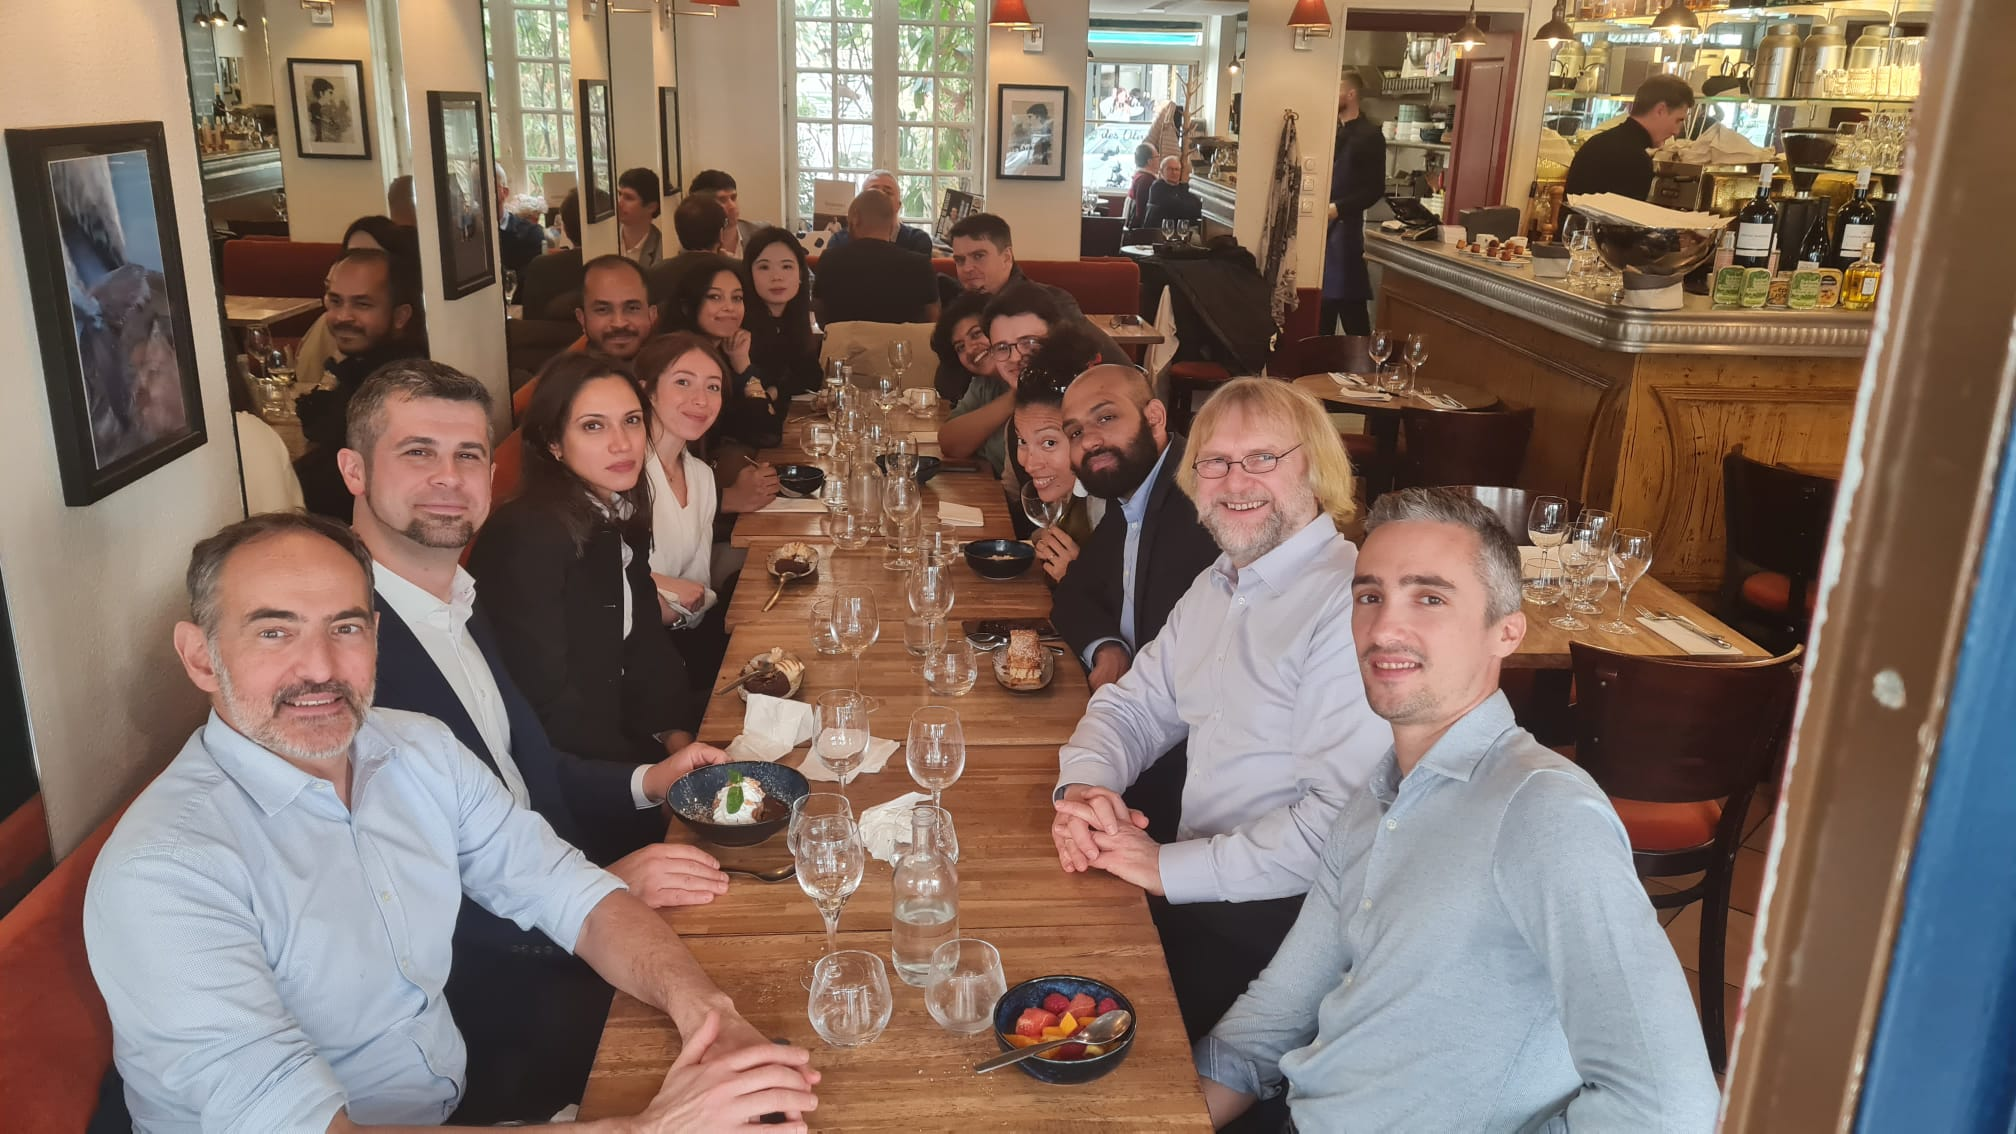
\includegraphics[width=.6\textwidth]{img/team.JPG}
  \caption{Équipe de parsienne}
\end{figure}
\end{frame}

% ==================================================================
\section{Épargne excédentaire}
\sectionpage
%###
\begin{frame}{Principaux objectifs}
  Intérêt du projet :
  \begin{itemize}
    \item Impact de la pandémie sur l'épargne des ménages en Europe + US ? 
    \item Accumulation d'une épargne dite excédentaire ? 
    \item Suivi et principaux drivers de cette épargne ? 
    \item Différences entre pays ?  
  \end{itemize}
\end{frame}

%###
\begin{frame}{Définition et calcul de l'épargne excédentaire}
  Première définition donnée par le Bureau of Economic Analysis
  \begin{align*}
    &\textrm{Flow of savings} = \textrm{DPI} - \textrm{PCE} - \textrm{\textit{other outlays}} \\
    \hookrightarrow \quad &\textrm{Flow of \blue{\textit{excess}} savings} = \blue{\Delta} \textrm{DPI} - \blue{\Delta} \textrm{PCE} - \blue{\Delta} \textrm{\textit{other outlays}}
  \end{align*}
  Où: $\Delta \textrm{\textit{X}}$ est l'écart relativement à la tendance pré-pandémique 2015-19 (log-linéaire) \\ 
  \vspace{.3cm}
  Pour les pays européens, on approche la définition de l'OCDE du revenu disponible (DPI) par la définition de la Fed:
  \begin{align*}
    \textrm{DPI} \cong  \textrm{Compensation of E} + \textrm{Net property income} + \textrm{transfers} - \textrm{taxes}
  \end{align*}
  (Pour les US on a exactement les mêmes données que Aladangaly \& al.)
  \vspace{.3cm}
  \begin{itemize}
    \item Intérêt: flux par composante du revenu disponible
  \end{itemize}
\end{frame}

%###
\begin{frame}{Calcul de l'épargne excédentaire}
  \begin{figure}
    \centering
    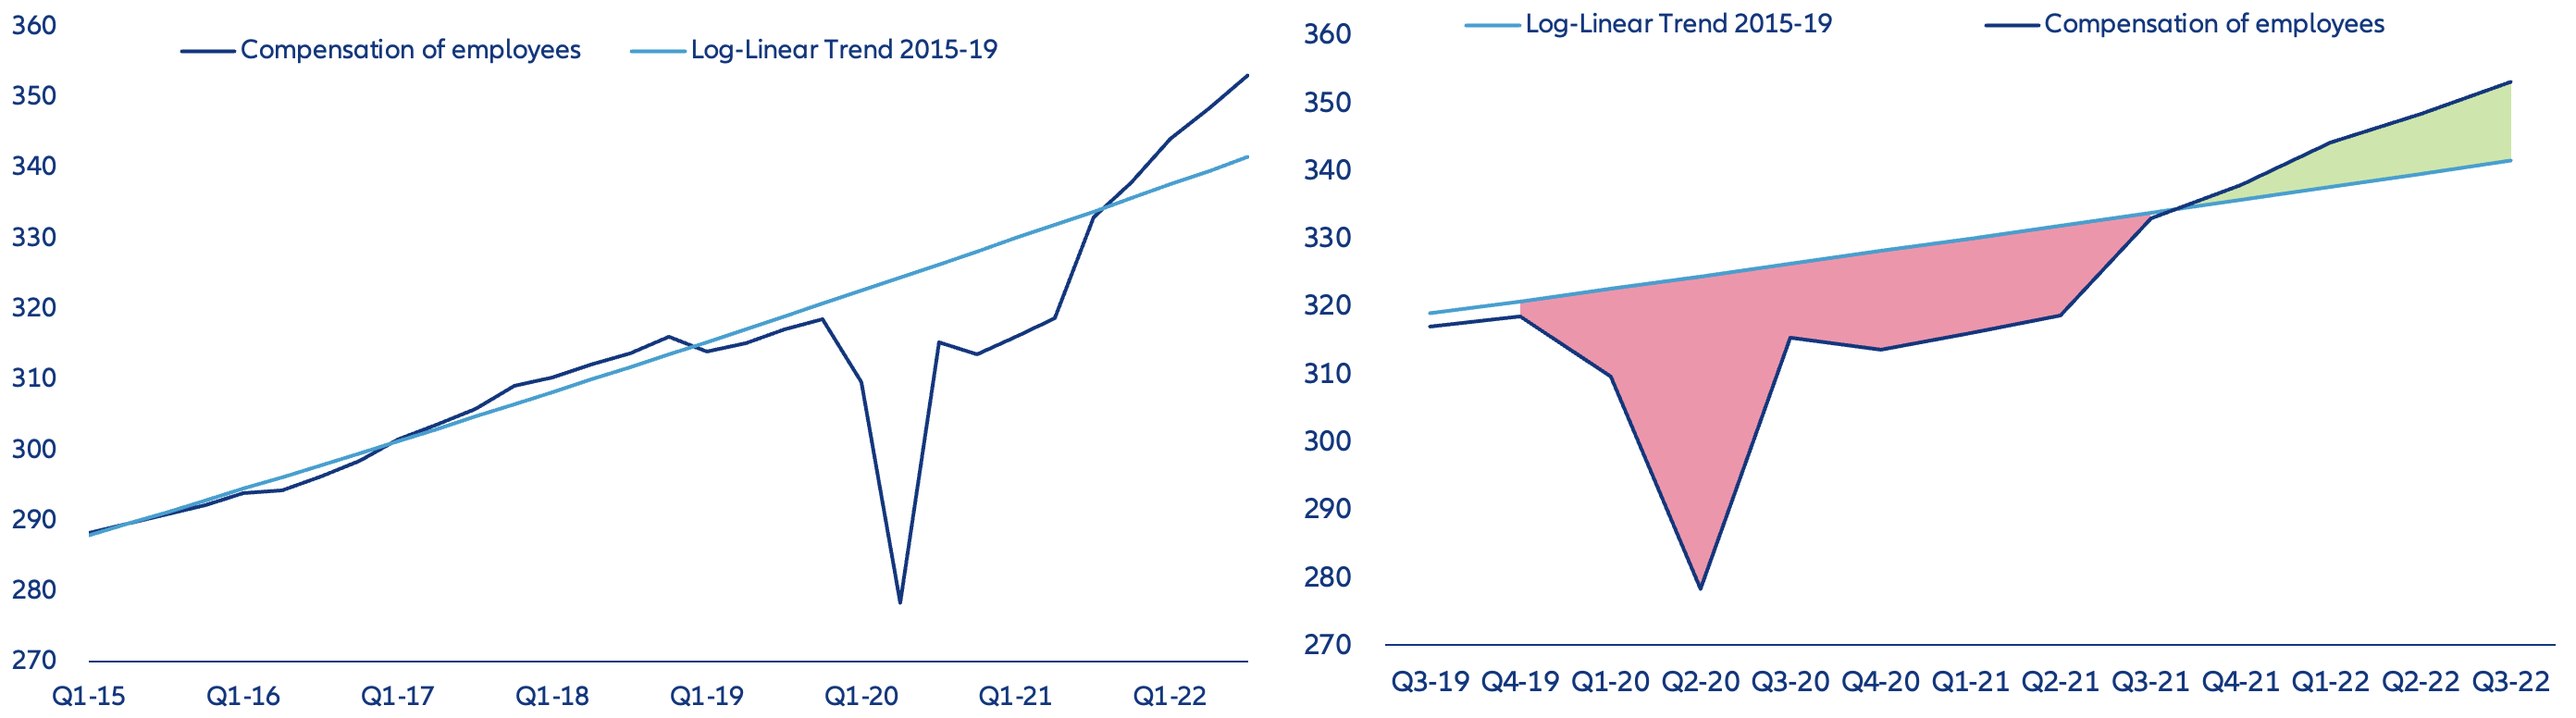
\includegraphics[width=1\textwidth]{img/excess_chart.png}
    \caption{Exemple - flux pour les compensation of employees: écart relatif à la tendance pré-pandémique (En rouge $\Delta Comp \leq 0$, en vert $\Delta Comp \geq  0$)}
  \end{figure}
\end{frame}

%###
\begin{frame}{Décomposition de l'épargne excédentaire par composante}
\end{frame}

%###
\begin{frame}{L'essentiel}
  Principaux résultats :
  \begin{itemize}
    \item X
    \item X
  \end{itemize}
  \vspace{.2cm}
  Retrospectivement :
  \begin{itemize}
    \item Décomposer PCE en bien et services
    \item 
  \end{itemize}
  \vspace{.2cm}
  Enseignements :
  \begin{itemize}
    \item Bases sur des grands aggrégats des comptes nationaux
    \item Importance des estimations d'épargne pour les ménages dans les débats  
    \item Difficulté d'obtenir de telles estimations
  \end{itemize}
\end{frame}

% ==================================================================
\section{Courbe de Phillips}
\begin{frame}[label=model]{Version dynamique de la courbe de Phillips}
  Forme générale de la courbe de Phillips estimée [\textit{ARDL}]:
  \begin{equation*}
    \blue{\Delta wage_{t}} = c + \phi_{1}(L).\blue{\Delta wage_{t}} + \phi_{2}(L).\blue{\Delta CPI_{t}} + \phi_{4}(L).\blue{\Delta slack_{t}} + \phi_{3}(L).\blue{prod_{t}} + \theta^{T}.\gamma + \epsilon_{t}
  \end{equation*}
  avec:
  \begin{itemize}
    \item $L$ l'opérateur retard
    \item Partie autoregressive: $\phi_{1}(L) = \sum_{k=\mathbf{1}}^{\mathbf{W}}\alpha_k L^{k}$ 
    \item Variables explicatives:
    \begin{itemize}
      \item $\phi_{2}(L) = \sum_{k=0}^{\mathbf{Q}}\beta_k^{(CPI)} L^{k}$
      \item $\phi_{3}(L) = \sum_{k=0}^{\mathbf{S}}\beta_k^{(slack)} L^{k}$
      \item $\phi_{4}(L) = \sum_{k=0}^{\mathbf{P}}\beta_k^{(prod)} L^{k}$
    \end{itemize}
    \item $\gamma$ un vecteur de variables binaires (Covid,GFC)
    \item $\epsilon_{t}$ terme d'erreur
  \end{itemize}
\end{frame}

\begin{frame}[label=est]{Model selection : slack}
  Au maximum : $W\in[1;6]\ \textrm{et} \left\{Q,S,P\right\}\in[0;6]^{3}$
\end{frame}

\begin{frame}{L'essentiel}
  Principaux résultats :
  \begin{itemize}
    \item X
    \item X
  \end{itemize}
  \vspace{.2cm}
  Retrospectivement :
  \begin{itemize}
    \item jsp
    \item 
  \end{itemize}
  \vspace{.2cm}
  Enseignements :
  \begin{itemize}
    \item jsp
    \item 
  \end{itemize}
\end{frame}

% ==================================================================
\section{Conclusion}
\begin{frame}{Publications}
  \begin{figure}
   \begin{columns}[c]
    \begin{column}{0.3\textwidth}
      \centering
      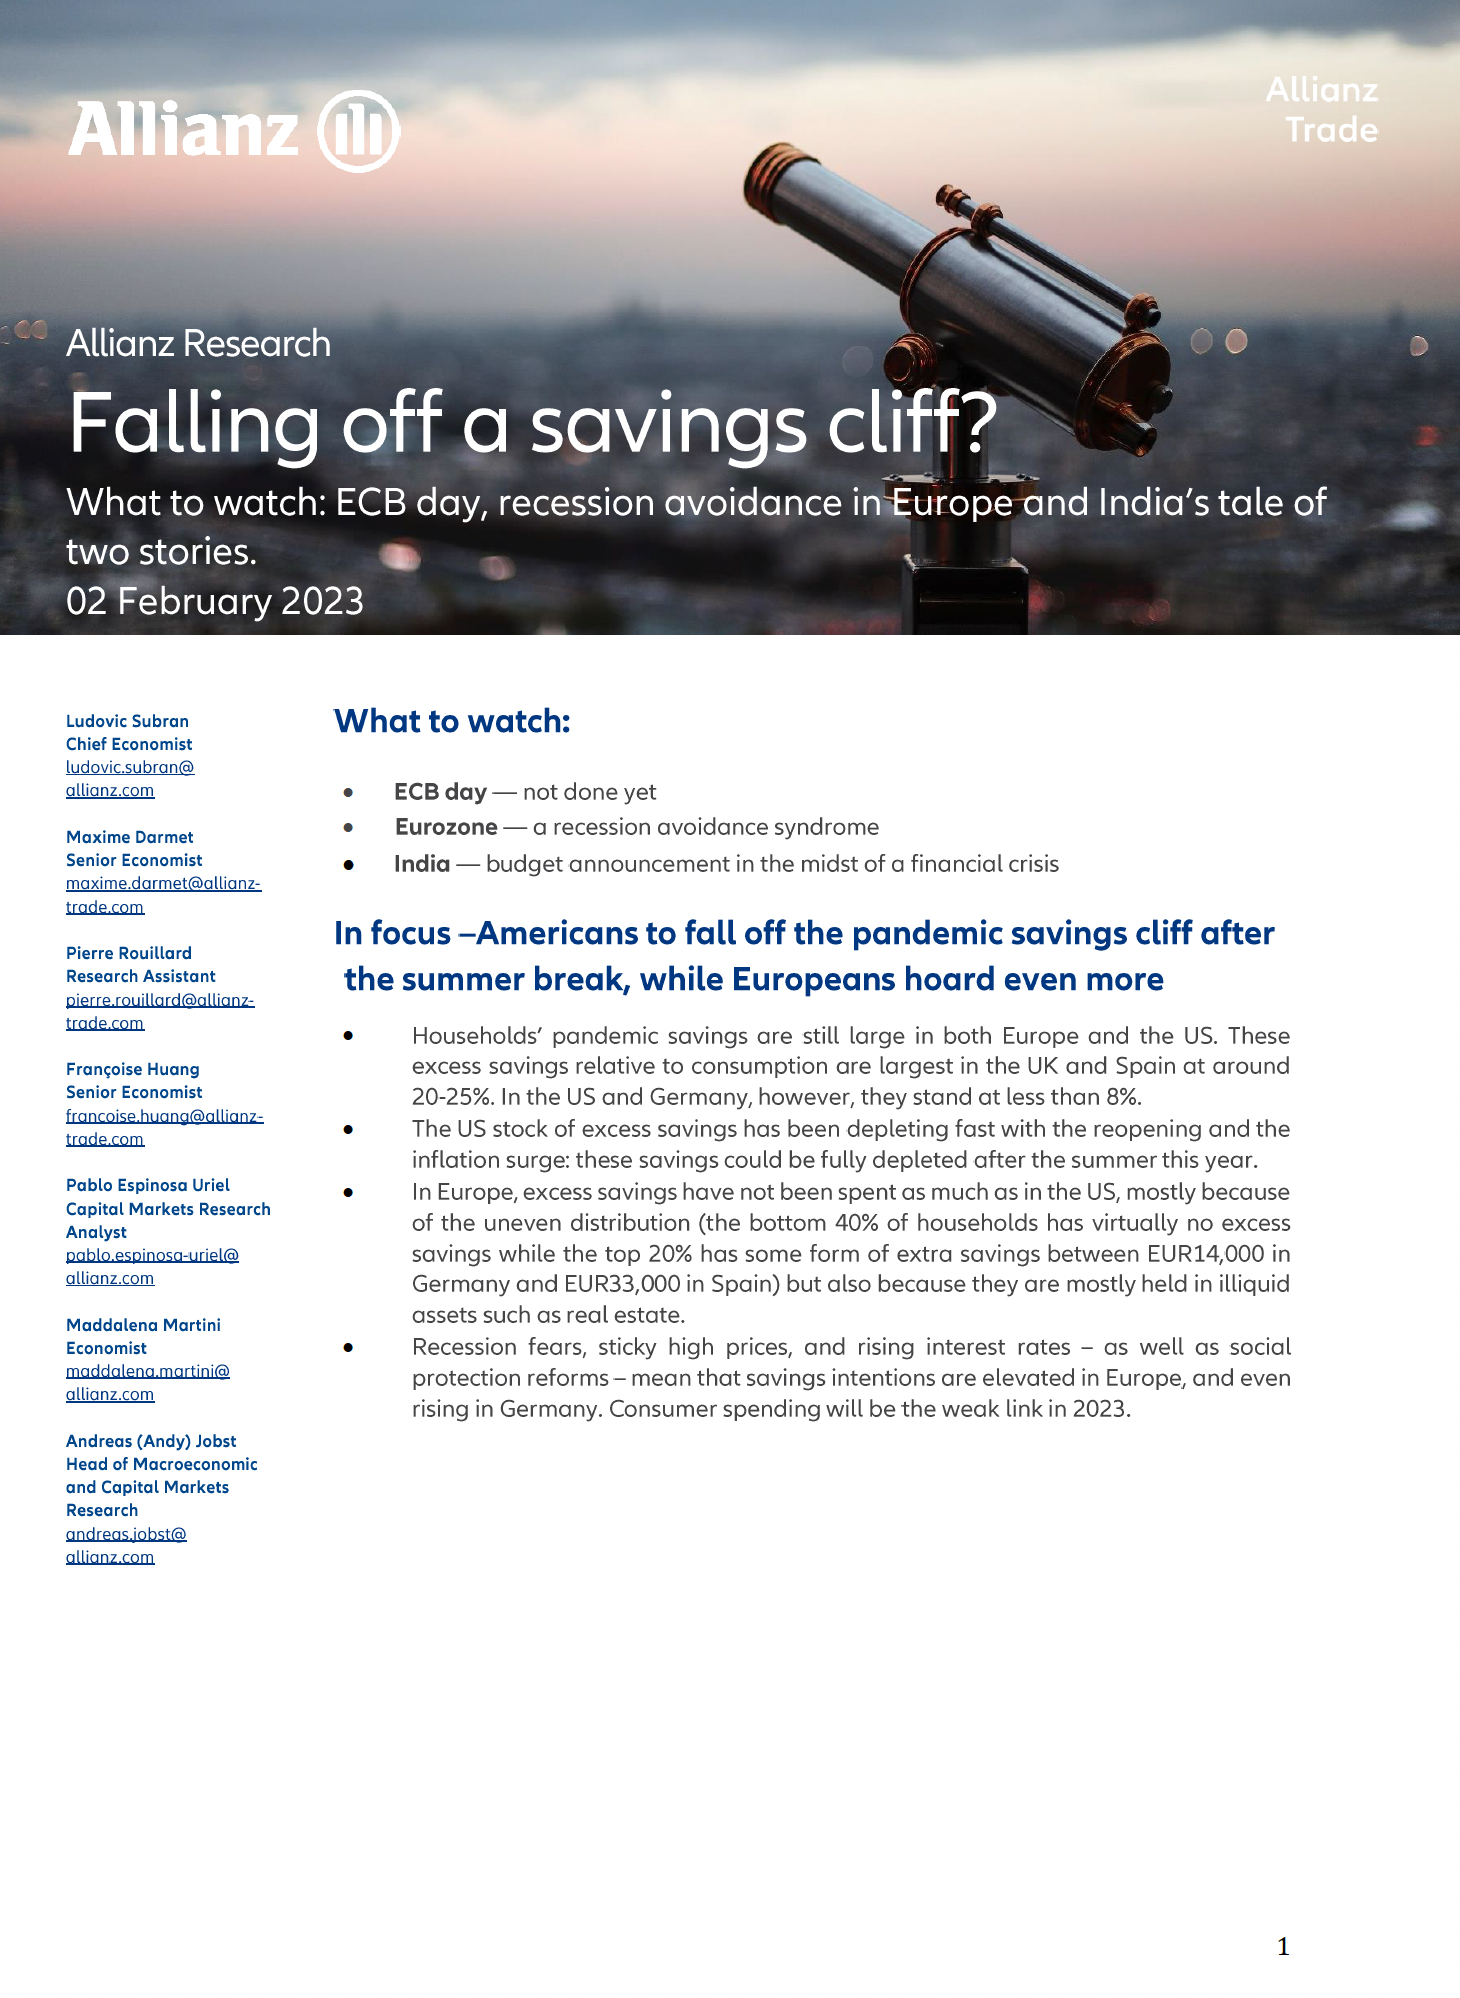
\includegraphics[width=1.3\textwidth]{img/az1.png}
    \end{column}
    \begin{column}{0.3\textwidth}
      \centering
      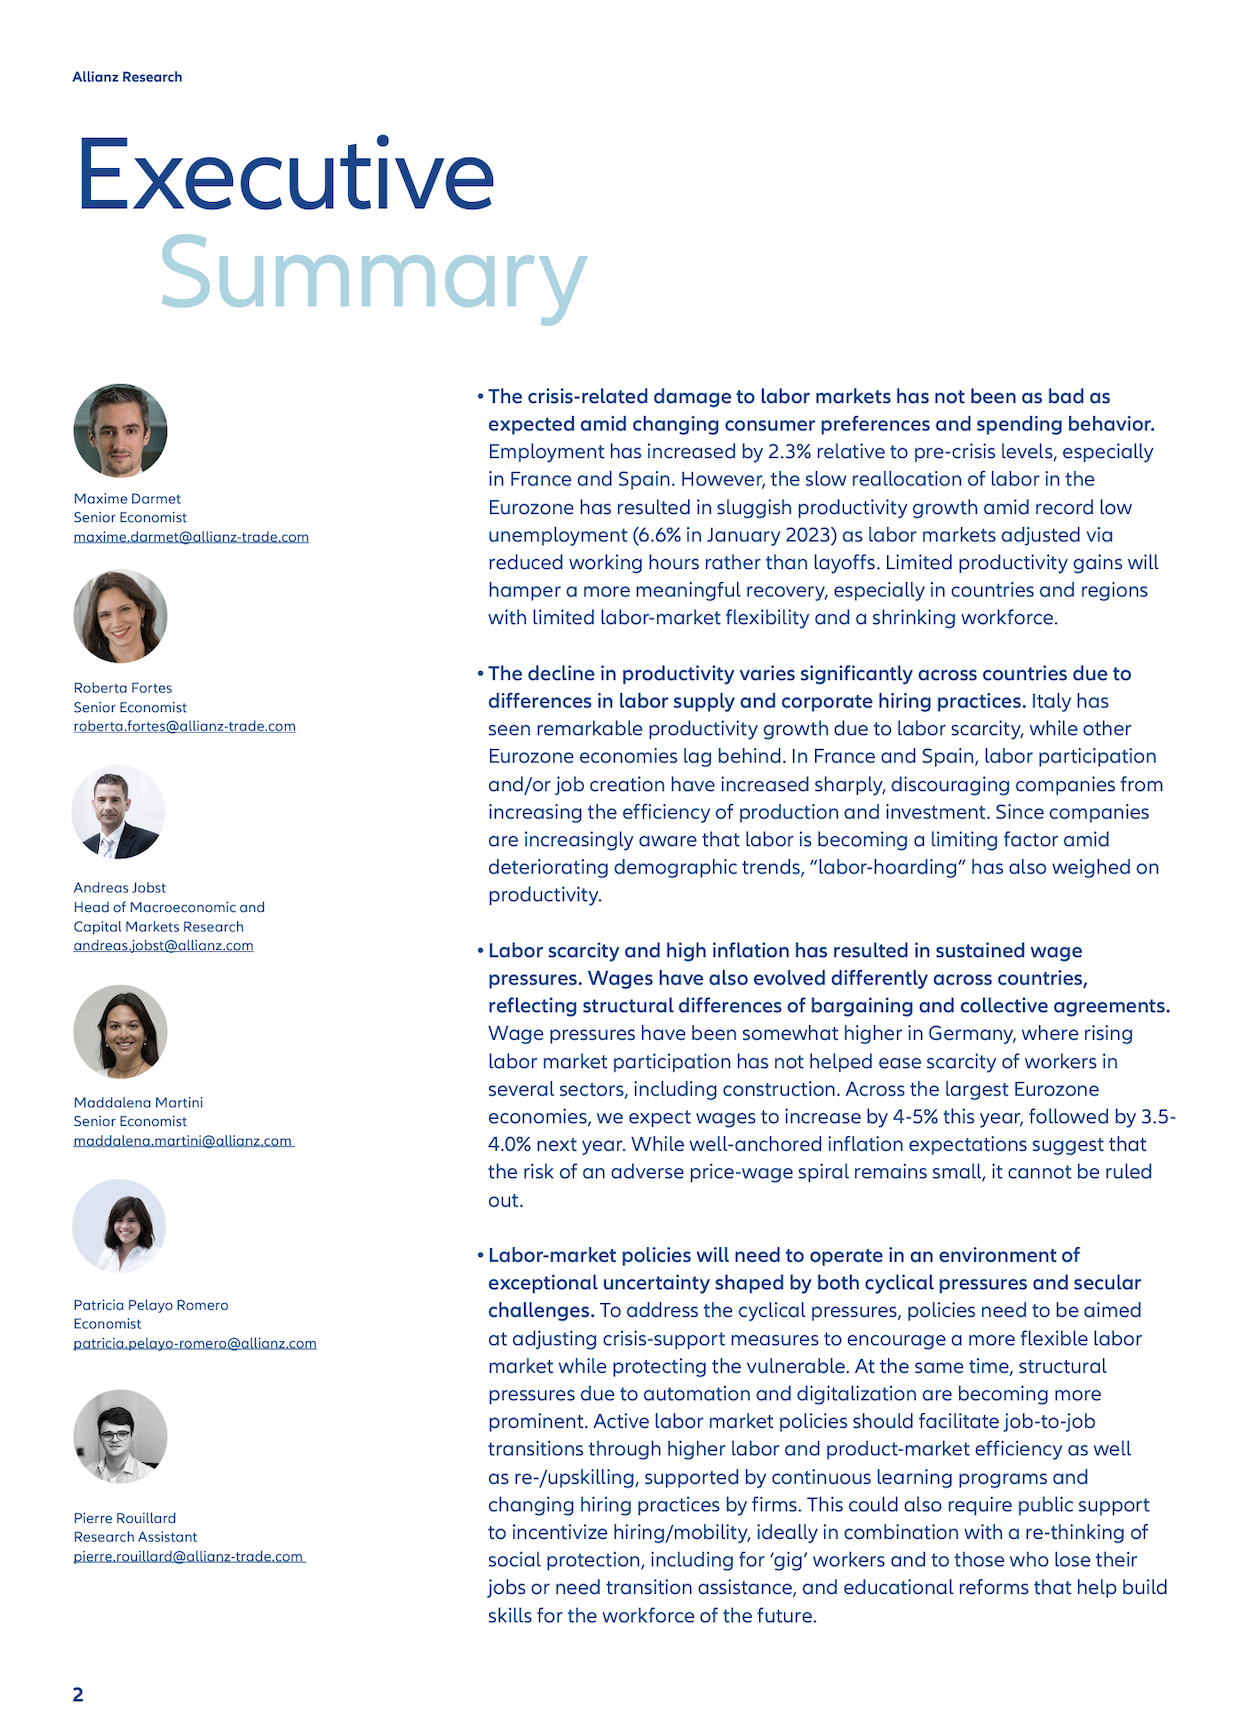
\includegraphics[width=1.3\textwidth]{img/az2.png}
    \end{column}
    \end{columns}
    \caption{Extraits des publications présentées (LHS: savings, RHS: wage)}
  \end{figure}
  \end{frame}

% -----------
\begin{frame}
 \begin{center}
		{\Huge Merci!}\\
		\bigskip\bigskip % Vertical whitespace
		{\LARGE pierre.rouillard@ensae.fr}
	\end{center}
\end{frame}

\end{document}